% $Header: /cvsroot/latex-beamer/latex-beamer/solutions/generic-talks/generic-ornate-15min-45min.en.tex,v 1.5 2007/01/28 20:48:23 tantau Exp $

\documentclass{beamer}

% This file is a solution template for:

% - Giving a talk on some subject.
% - The talk is between 15min and 45min long.
% - Style is ornate.



% Copyright 2004 by Till Tantau <tantau@users.sourceforge.net>.
%
% In principle, this file can be redistributed and/or modified under
% the terms of the GNU Public License, version 2.
%
% However, this file is supposed to be a template to be modified
% for your own needs. For this reason, if you use this file as a
% template and not specifically distribute it as part of a another
% package/program, I grant the extra permission to freely copy and
% modify this file as you see fit and even to delete this copyright
% notice. 


\mode<presentation>
{
  \usetheme{Warsaw}
  % or ...

  \setbeamercovered{transparent}
  % or whatever (possibly just delete it)
}


\usepackage[spanish,english]{babel}
% or whatever

%\usepackage[latin1]{inputenc}
\usepackage[utf8]{inputenc}
% or whatever

\usepackage{times}
\usepackage[T1]{fontenc}
% Or whatever. Note that the encoding and the font should match. If T1
% does not look nice, try deleting the line with the fontenc.

\usepackage{amsmath}
\usepackage{eurosym}  
\usepackage{graphicx} 
\usepackage{float}
\usepackage{booktabs}
\usepackage{multicol}

% path to directories containing images
\graphicspath{{./logos/}{./figures/}{./diagrams/}} % Edit this to your
                                % needs. Only logos is really required
                                % when you generate your own content.


\title[Manual de referencia para el desarrollo de robots de Eurobot] % (optional, use only with long paper titles)
{Manual de referencia para el desarrollo de robots de Eurobot}

\subtitle
{Trabajo Fin de Carrera} % (optional)

\author[Javier Baliñas Santos] % (optional, use only with lots of authors)
{
	Javier Baliñas Santos\\ 
	Director: Julio Pastor Mendoza
}
% - Use the \inst{?} command only if the authors have different
%   affiliation.

\institute[Universities of Somewhere and Elsewhere] % (optional, but mostly needed)
{
	\textsc{Departamento de Electrónica}\\
	\vspace{.5cm} 
	
\includegraphics[height=1cm]{logoUAHazul}\\ 
	\textsc{Universidad de Alcalá}
}
% - Use the \inst command only if there are several affiliations.
% - Keep it simple, no one is interested in your street address.

\date[29 de septiembre de 2016] % (optional)
{29 de septiembre de 2016}

\subject{Talks}
% This is only inserted into the PDF information catalog. Can be left
% out. 

% If you have a file called "university-logo-filename.xxx", where xxx
% is a graphic format that can be processed by latex or pdflatex,
% resp., then you can add a logo as follows:

% \pgfdeclareimage[height=0.5cm]{university-logo}{university-logo-filename}
% \logo{\pgfuseimage{university-logo}}



% Delete this, if you do not want the table of contents to pop up at
% the beginning of each subsection:
%\AtBeginSubsection[]
%{
%  \begin{frame}<beamer>{Cont}
%    \tableofcontents[currentsection,currentsubsection]
%  \end{frame}
%}

\AtBeginSection[]
{
  \begin{frame}<beamer>
    %\frametitle{Contenido} 
    %\setcounter{tocdepth}{2}
    \tableofcontents[currentsection]
  \end{frame}
}


% If you wish to uncover everything in a step-wise fashion, uncomment
% the following command: 

%\beamerdefaultoverlayspecification{<+->}


\begin{document}

\begin{frame}
  \titlepage
\end{frame}

\begin{frame}{Contenido}
	\setcounter{tocdepth}{1}
	\tableofcontents%[pausesections]
  	% You might wish to add the option [pausesections]
\end{frame}


% Since this a solution template for a generic talk, very little can
% be said about how it should be structured. However, the talk length
% of between 15min and 45min and the theme suggest that you stick to
% the following rules:  

% - Exactly two or three sections (other than the summary).
% - At *most* three subsections per section.
% - Talk about 30s to 2min per frame. So there should be between about
%   15 and 30 frames, all told.

%\section{Example}

%\subsection[Short First Subsection Name]{First Subsection Name}

%\begin{frame}{Make Titles Informative. Use Uppercase Letters.}{Subtitles are optional.}
%  % - A title should summarize the slide in an understandable fashion
%  %   for anyone how does not follow everything on the slide itself.

%  \begin{itemize}
%  \item
%    Use \texttt{itemize} a lot.
%  \item
%    Use very short sentences or short phrases.
%  \end{itemize}
%\end{frame}

%\begin{frame}{Make Titles Informative.}

%  You can create overlays\dots
%  \begin{itemize}
%  \item using the \texttt{pause} command:
%    \begin{itemize}
%    \item
%      First item.
%      \pause
%    \item    
%      Second item.
%    \end{itemize}
%  \item
%    using overlay specifications:
%    \begin{itemize}
%    \item<3->
%      First item.
%    \item<4->
%      Second item.
%    \end{itemize}
%  \item
%    using the general \texttt{uncover} command:
%    \begin{itemize}
%      \uncover<5->{\item
%        First item.}
%      \uncover<6->{\item
%        Second item.}
%    \end{itemize}
%  \end{itemize}
%\end{frame}


\section{Introducción}

\begin{frame}{La competición Eurobot}
\begin{center}
\alt<1>{
\includegraphics[width=.6\textwidth]{eurobot2}}{}
\alt<2>{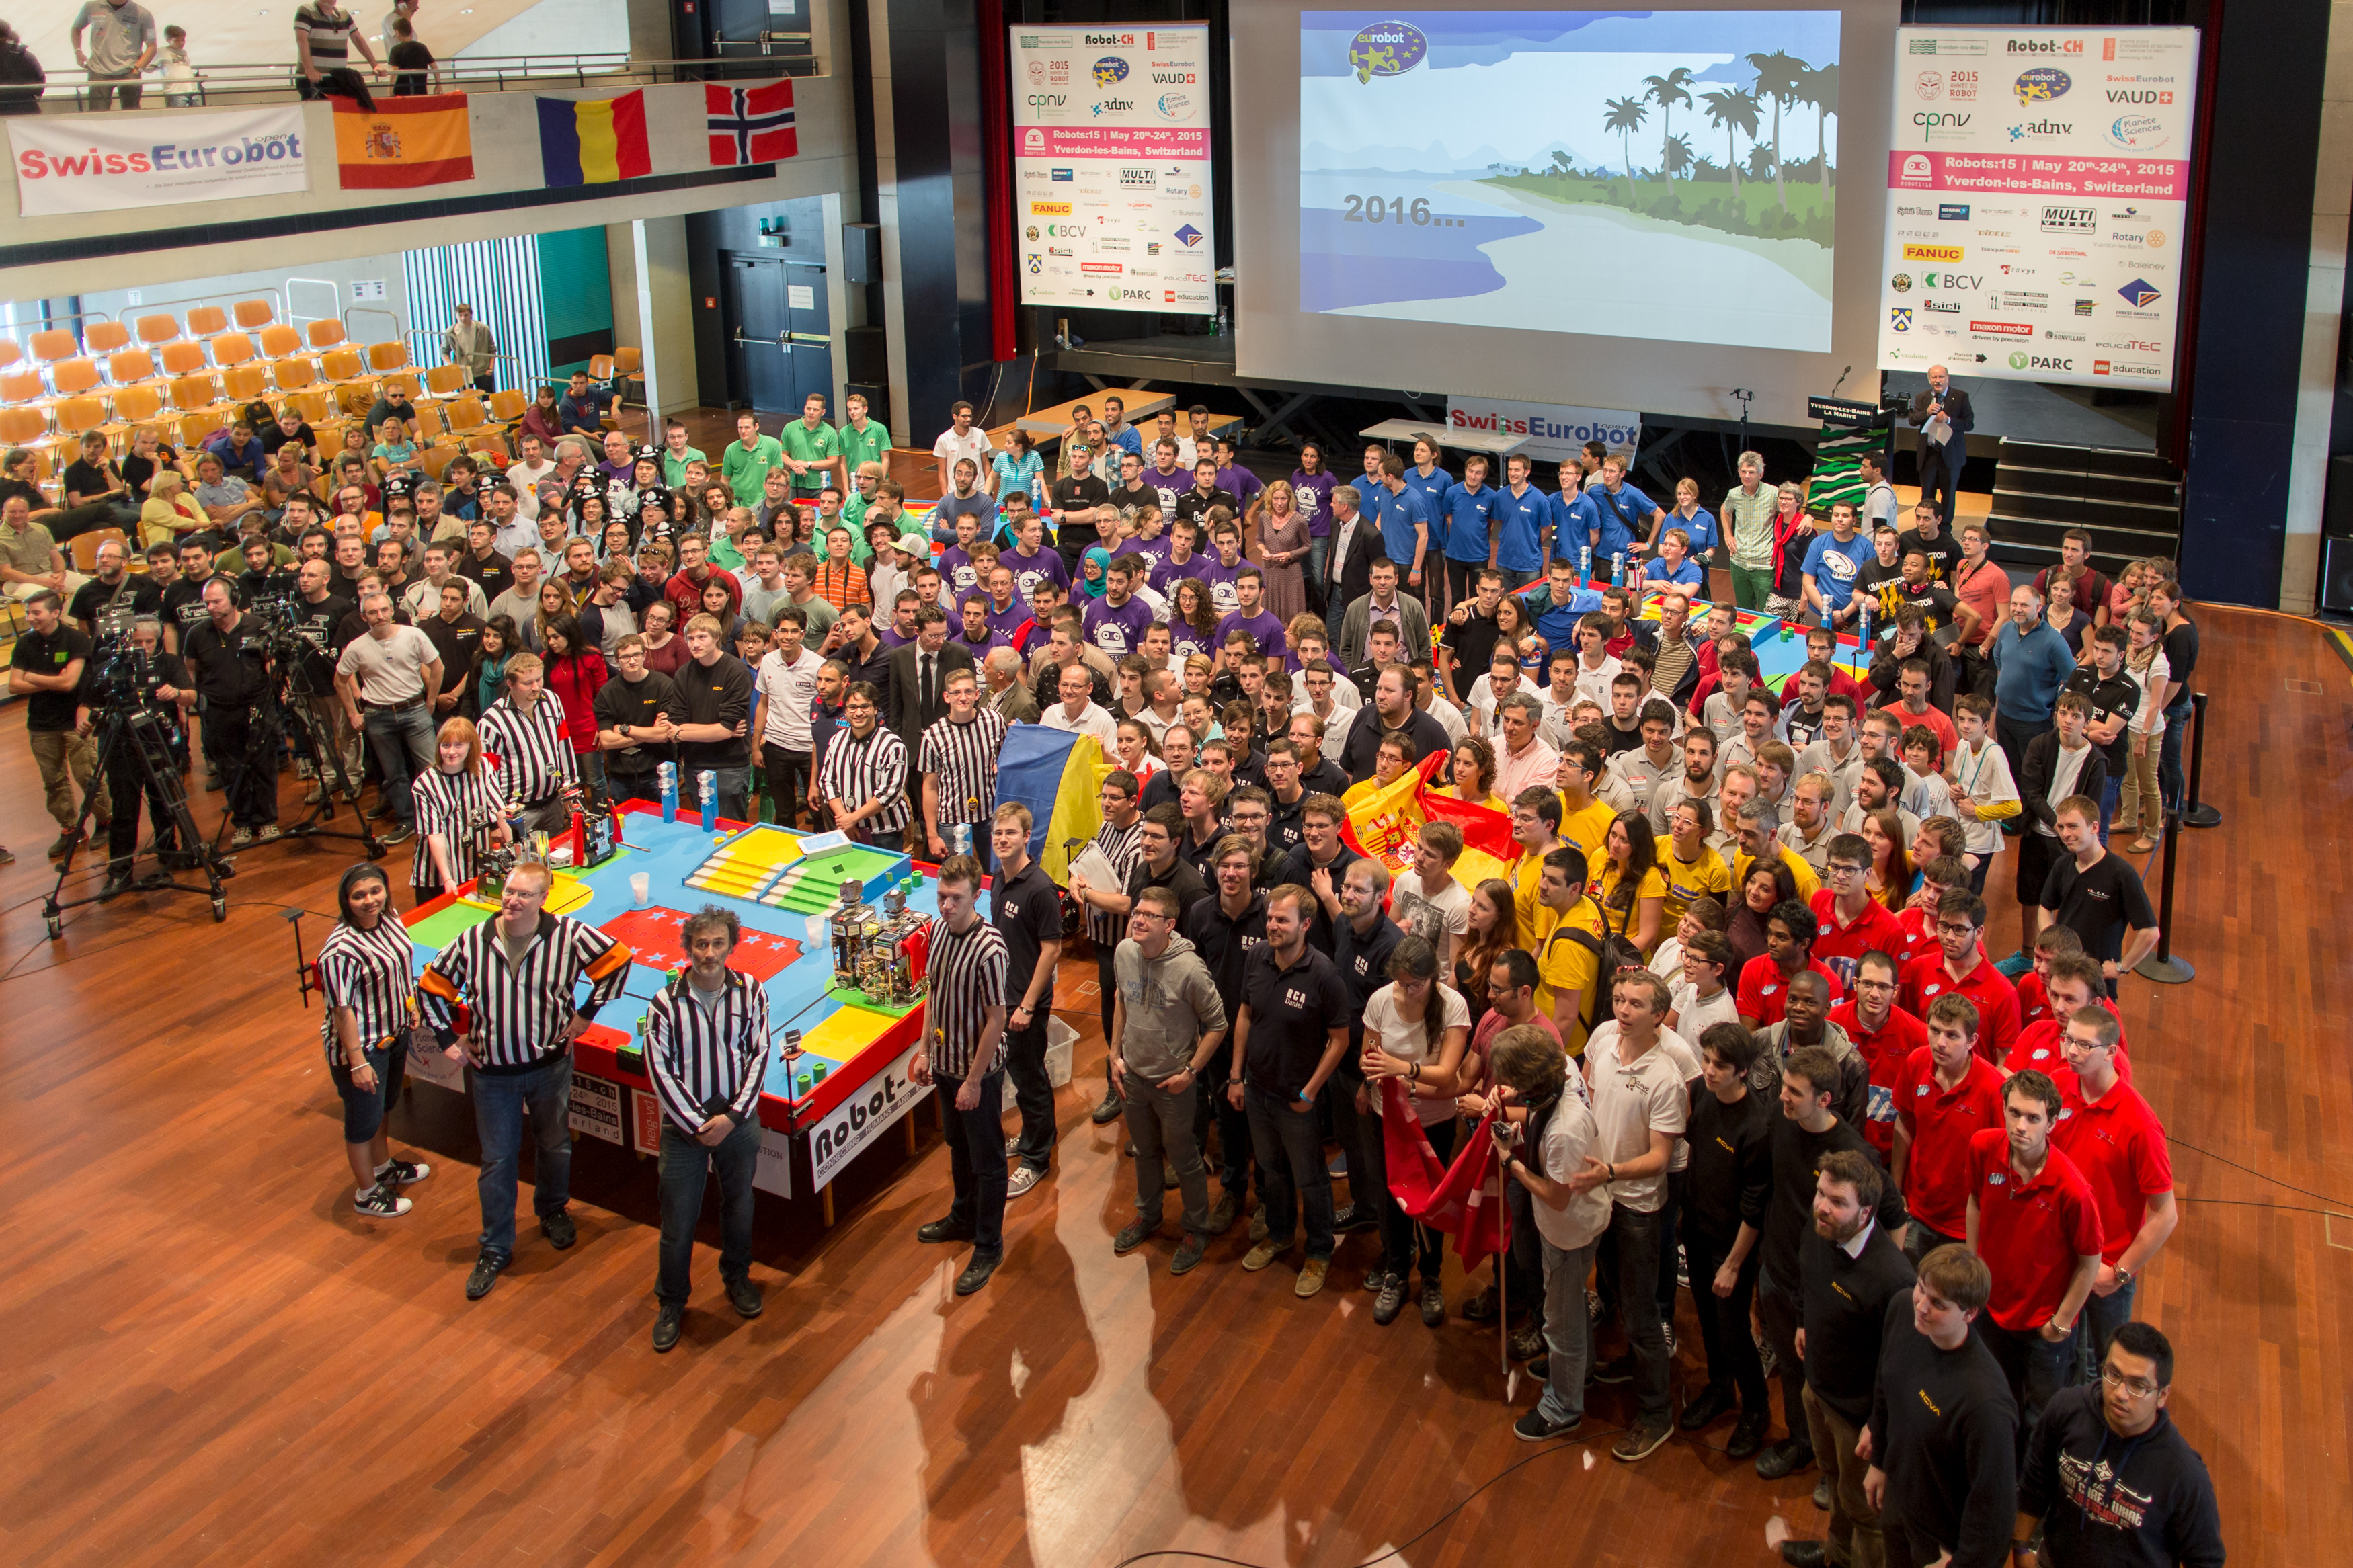
\includegraphics[width=.9\textwidth]{eurobot_family}}{}
\end{center}
\end{frame}

\begin{frame}{Eurobotics Engineering}

\begin{columns}
\column{.5\textwidth}
\centering

\includegraphics[width=\textwidth]{bombona}

\column{.5\textwidth}
\centering
\alt<1>{
\includegraphics[width=\textwidth]{arc_logo_cartel}\\
		
\includegraphics[width=\textwidth]{logotexto1}}{}

\alt<2>{
\includegraphics[width=\textwidth]{Logo_depeca_Grande_rojo_2_150ppp}}{}

\alt<3>{
\includegraphics[width=\textwidth]{AYTO-COSLADA}\\
		
\includegraphics[width=\textwidth]{ayudas_hidraulicas}\\
		\vspace{.2cm}
		
\includegraphics[width=.7\textwidth]{splashscreen_logo}}{}

\end{columns}
\end{frame}

\begin{frame}{Motivación}

\begin{itemize}
\item Afición a la robótica, electrónica y los sistemas embebidos
\item Inquietud Maker
\item Divulgación del conocimiento
\end{itemize}

\end{frame}


\section{El robot de Eurobot}
%\subsection{Especificaciones}

\begin{frame}{El juego y sus elementos}
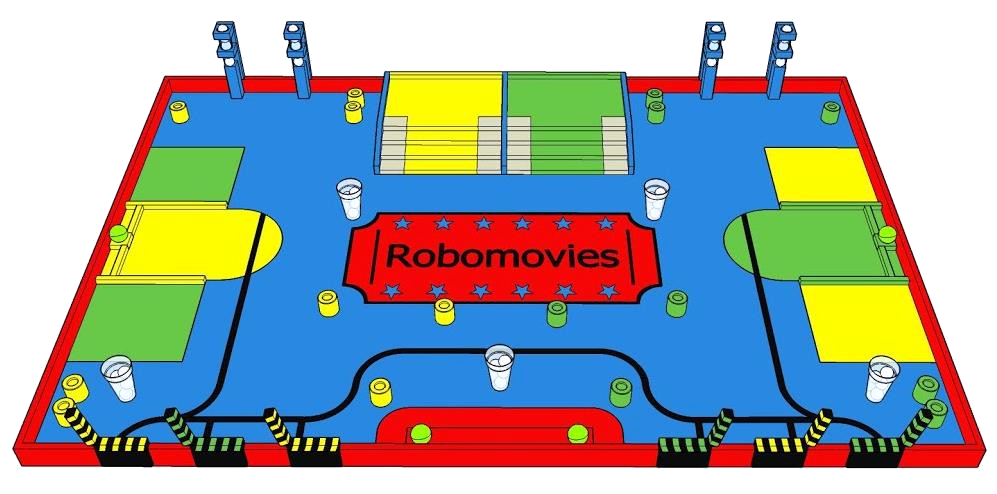
\includegraphics[width=.9\textwidth]{campo_2015}
\end{frame}

\begin{frame}{Los robots}
\begin{columns}
\column{.5\textwidth}

\begin{itemize}
\item Autónomo (90s)
\item Realizar acciones del juego
\item Evitar colisiones
\item Hasta 2 robots por equipo
\item Perímetro máximo 1,2/1.5m (70/90cm)
\item Altura máxima 35cm
\item Sistemas de balizas
\end{itemize}

\column{.5\textwidth}
\centering
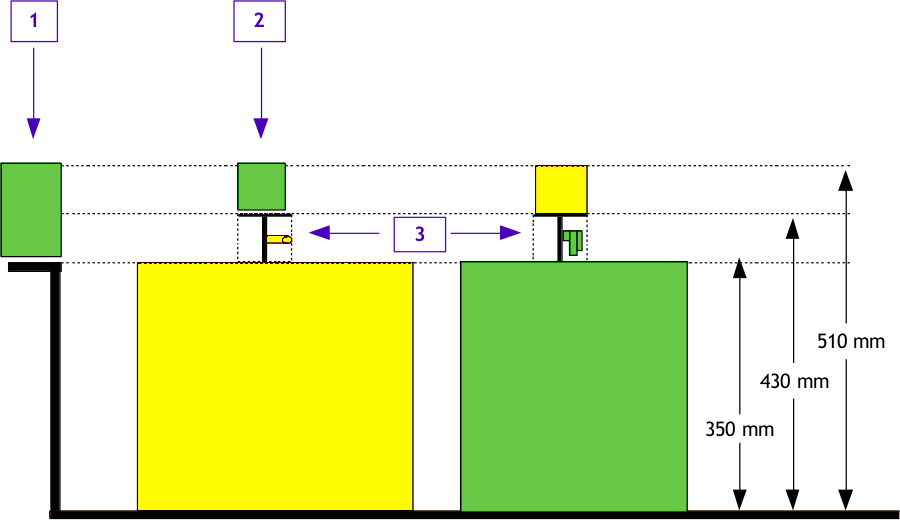
\includegraphics[width=\textwidth]{balizas_robots}
\end{columns}
\end{frame}


%\subsection{Funcionalidades}

\begin{frame}{Funcionalidades a desarrollar}

\alt<1> {
	\begin{enumerate}
	\item Estrategia de juego
	\item Evitación de obstáculos
	\item Comunicación entre robots
	\item Manipulación de elementos de juego
	\end{enumerate}
}{}

\alt<2>{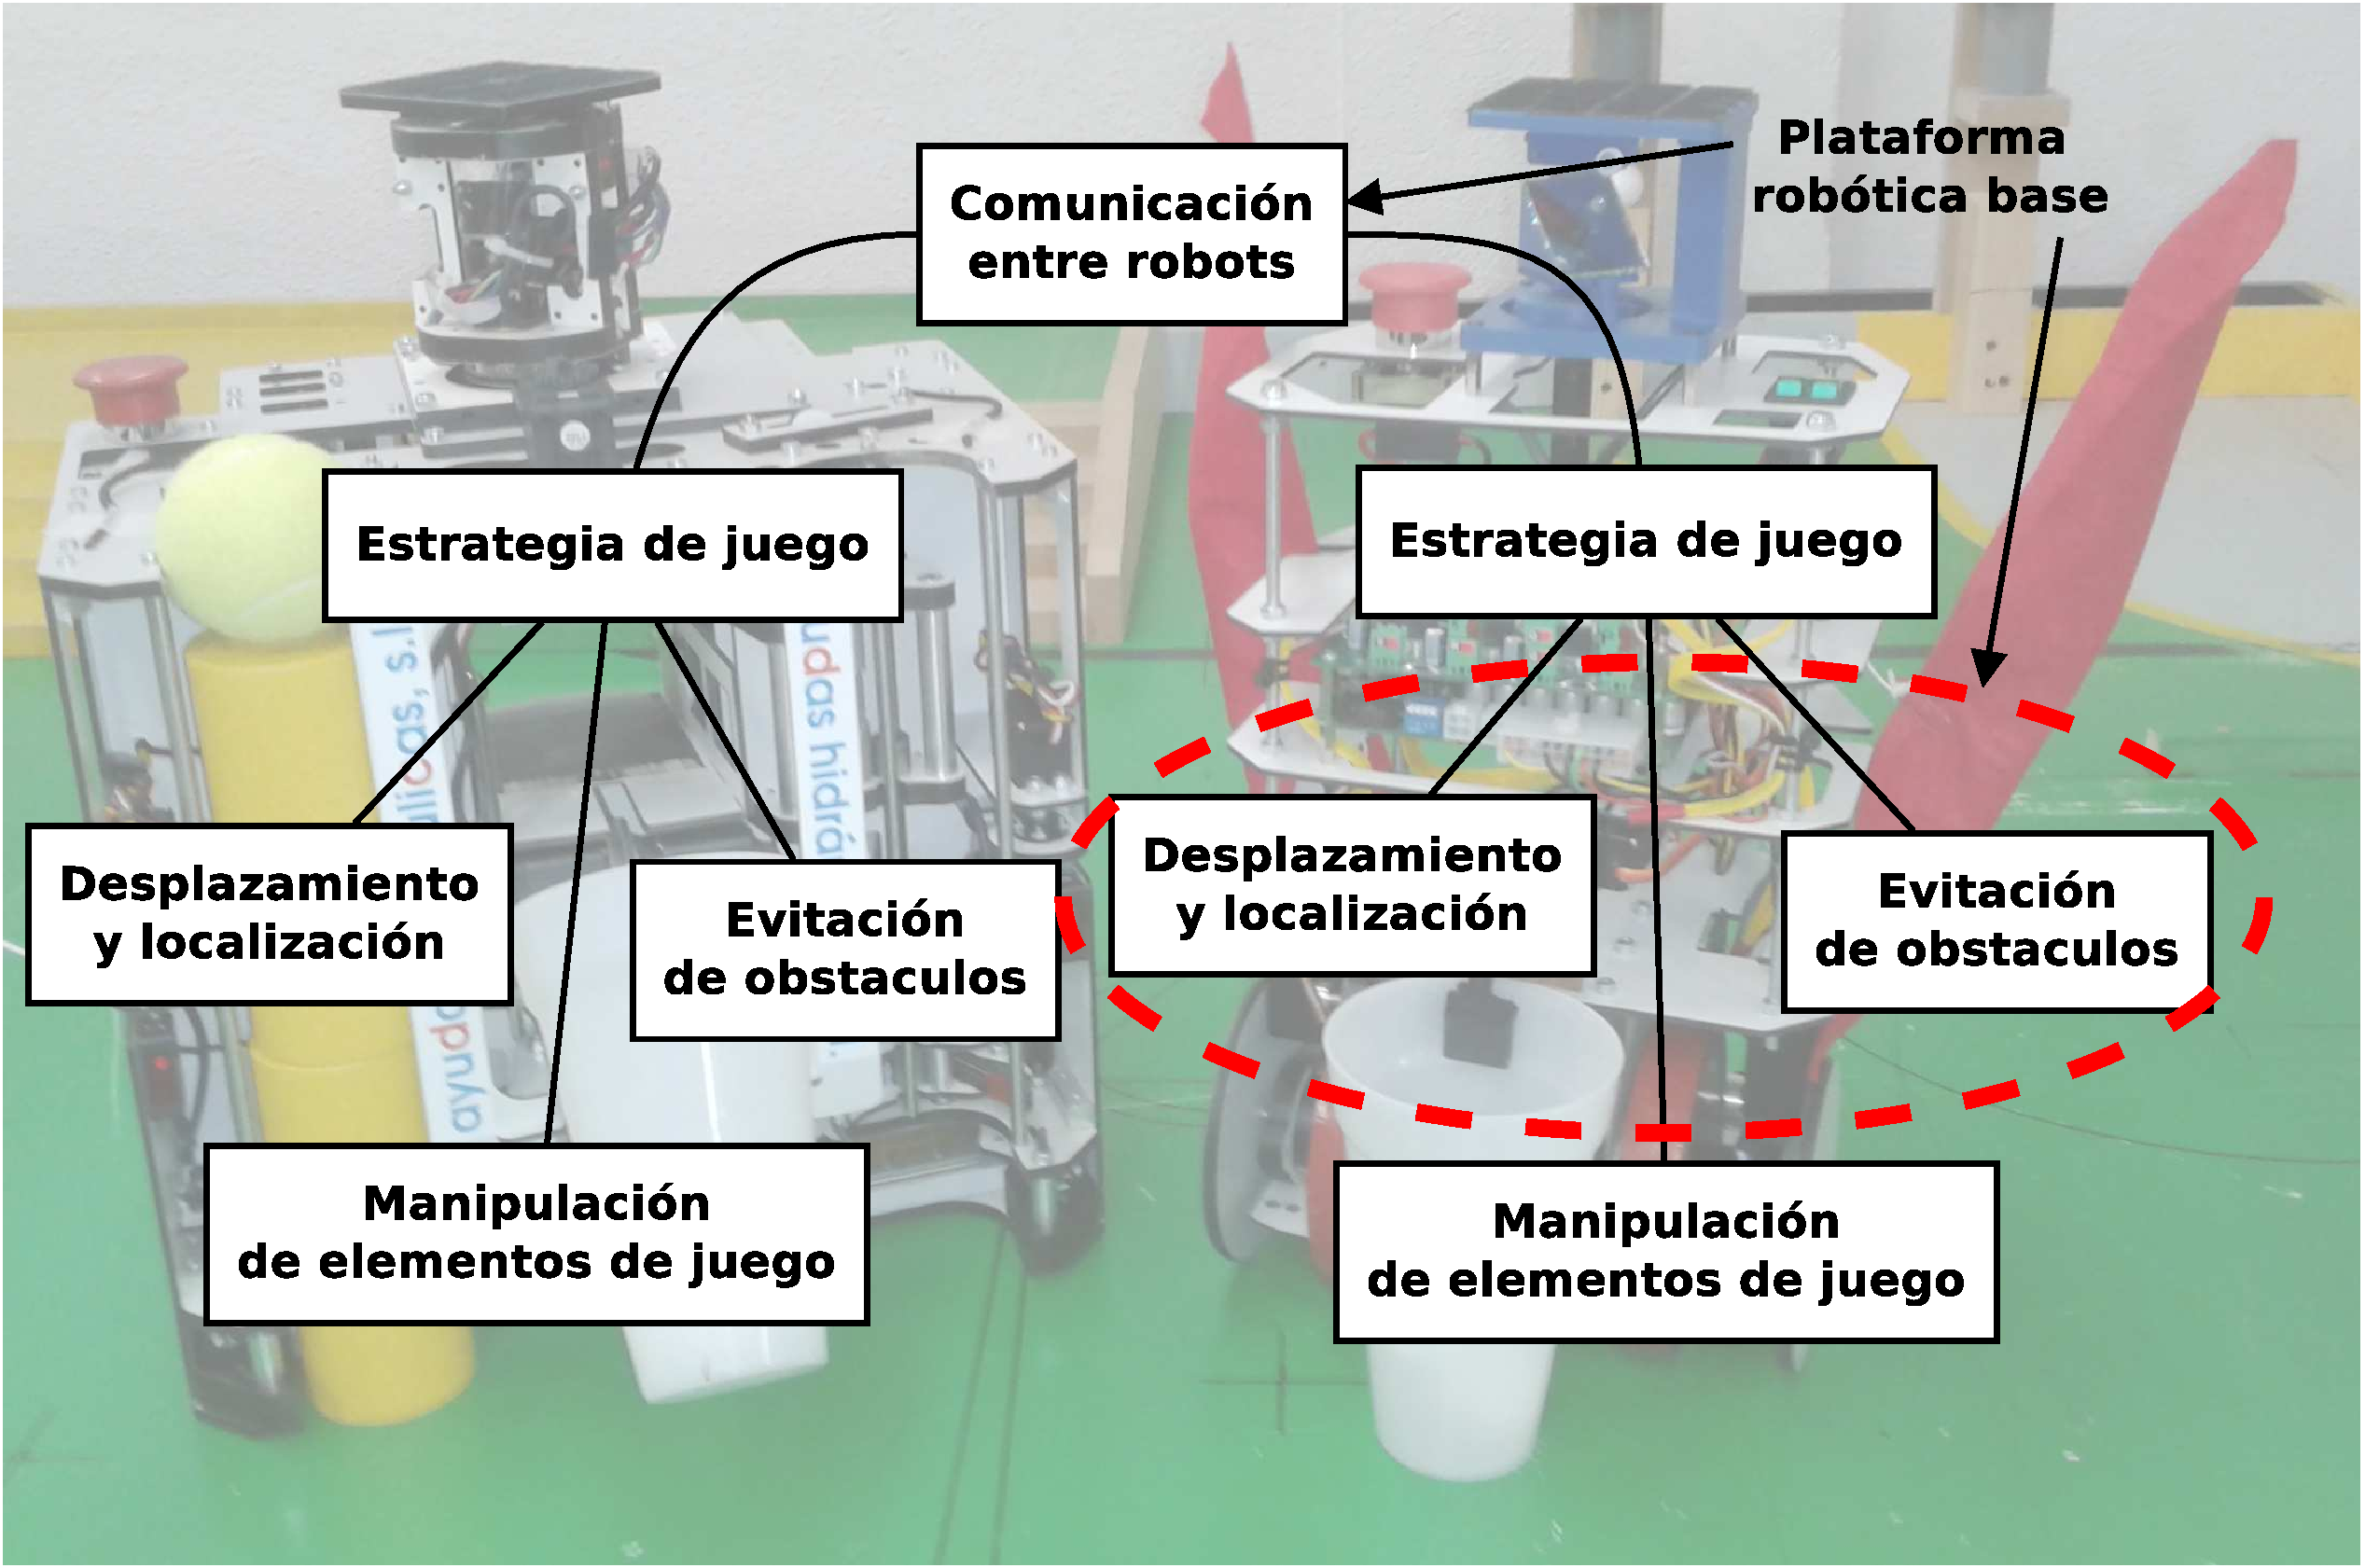
\includegraphics[width=.9\textwidth]{partes_robot_eurobot}}{}
\end{frame}

%\begin{frame}{Estrategia de juego}
%\includegraphics[width=\textwidth]{}
%\end{frame}

%\begin{frame}{Desplazamiento y localización}
%\includegraphics[width=\textwidth]{}
%\end{frame}

%\begin{frame}{Evitación de obstáculos}
%\alt<1>{\includegraphics[width=\textwidth]{}}{}
%\alt<1>{\includegraphics[width=\textwidth]{}}{}
%\alt<1>{\includegraphics[width=\textwidth]{}}{}
%\end{frame}

%\begin{frame}{Comunicación entre robots}
%\includegraphics[width=\textwidth]{}
%\end{frame}

%\begin{frame}{Manipulación de elementos de juego}
%\includegraphics[width=\textwidth]{}
%\end{frame}

%\subsection{Desarrollo}

\begin{frame}{Fases de desarrollo}
\end{frame}

%\begin{frame}{Diseño de la estrategia}
%\includegraphics[width=\textwidth]{}
%\end{frame}

%\begin{frame}{Prototipos y pruebas de concepto}
%\alt<1>{\includegraphics[width=\textwidth]{}
%		\includegraphics[width=\textwidth]{}}{}
%\alt<2>{\includegraphics[width=\textwidth]{}
%		\includegraphics[width=\textwidth]{}}{}
%\end{frame}




\section{Plataforma robótica base}
\subsection{Partes principlales}

\begin{frame}{Bloque motor, ruedas libres y electrónica}
\end{frame}

\begin{frame}{Puntos de apoyo}
\end{frame}

\begin{frame}{Detección de obstáculos y oponentes}
\end{frame}

\begin{frame}{Ruedas libres}
%\alt<1>{\includegraphics[width=\textwidth]{}}{}
%\alt<2>{\includegraphics[width=\textwidth]{}}{}
\end{frame}



\subsection{Dinámica}
\subsection{Control de posición}
\subsection{Odometría}

\section{Desarrollo HW y SW}

\appendix
\section*{Conclusiones}

\begin{frame}{Conclusiones}

  % Keep the summary *very short*.
  \begin{itemize}
  \item
    The \alert{first main message} of your talk in one or two lines.
  \item
    The \alert{second main message} of your talk in one or two lines.
  \item
    Perhaps a \alert{third message}, but not more than that.
  \end{itemize}
  
  % The following outlook is optional.
  \vskip0pt plus.5fill
  \begin{itemize}
  \item
    Outlook
    \begin{itemize}
    \item
      Something you haven't solved.
    \item
      Something else you haven't solved.
    \end{itemize}
  \end{itemize}
\end{frame}


\end{document}


